\begin{frame}
\frametitle{Dispersion}
Frequenzabhängige Ausbreitungsgeschwindigkeit von Wellen 
\begin{equation*}
  f(\kappa,\omega)=0.
\end{equation*}
\begin{figure}
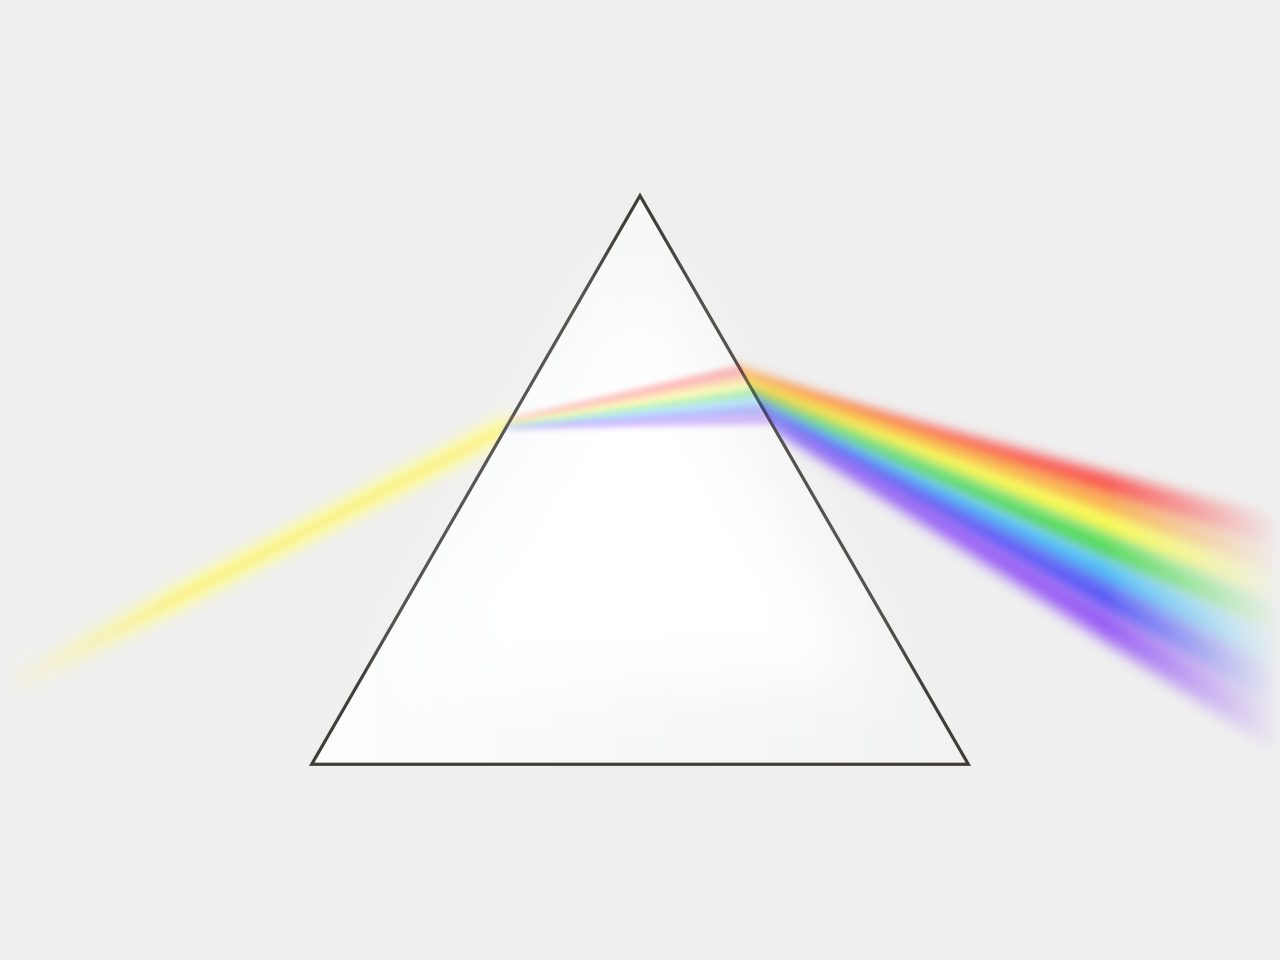
\includegraphics[width=0.475\textwidth]{fig_img/wikipedia_dispersion.png}
\caption*{Dispersion im Prisma erzeugt ein Farbspektrum \href{https://commons.wikimedia.org/w/index.php?curid=3728535}{[Suidroot]}}
\end{figure}
\end{frame}


\begin{frame}
\frametitle{Exkurs -- Schwebung}
\only<1>{
\begin{figure}
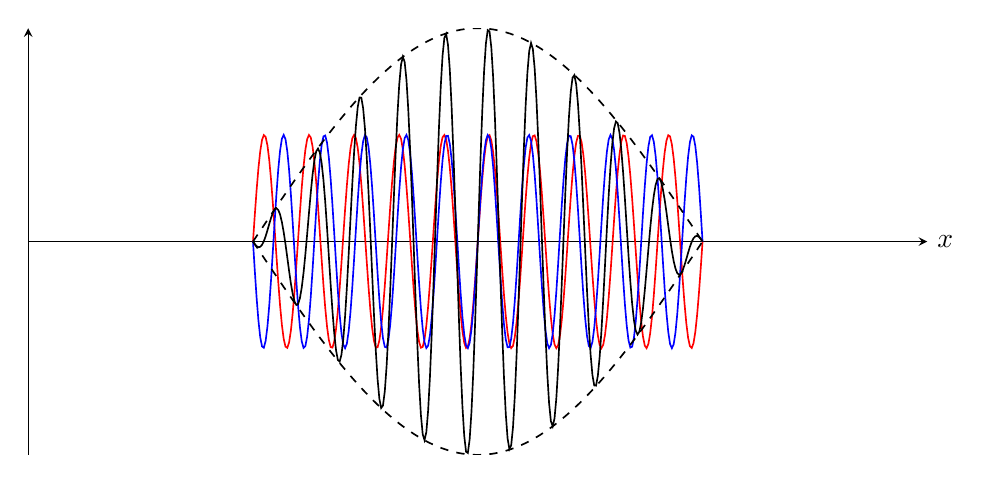
\begin{tikzpicture}
\begin{axis}[
    width=13cm, 
    height=7cm,
    axis x line=center, 
    axis y line=middle, 
    xlabel={$x$},
     x label style={at={(current axis.right of origin)}, right},
    samples=250,
    ymin=-2, ymax=2,
    xmin=0, xmax=20,
    domain=5:15,
    ticks=none
]
\addplot [mark=none, semithick, red] {sin(deg(2*pi*x))};
\addplot [mark=none, semithick, blue] {sin(deg(2*pi*x*1.1))};
\addplot [mark=none, semithick, black] {sin(deg(2*pi*x))+sin(deg(2*pi*x*1.1))};
\addplot [mark=none, semithick, dashed] { 2*cos(deg(2*pi*x*0.05))};
\addplot [mark=none, semithick, dashed] {-2*cos(deg(2*pi*x*0.05))};
\end{axis}
\end{tikzpicture}

\caption*{Die Überlagung naheliegender Frequenzen liegt unter einer Einhüllenden}
\end{figure}
} %only

\only<2>{
\begin{figure}
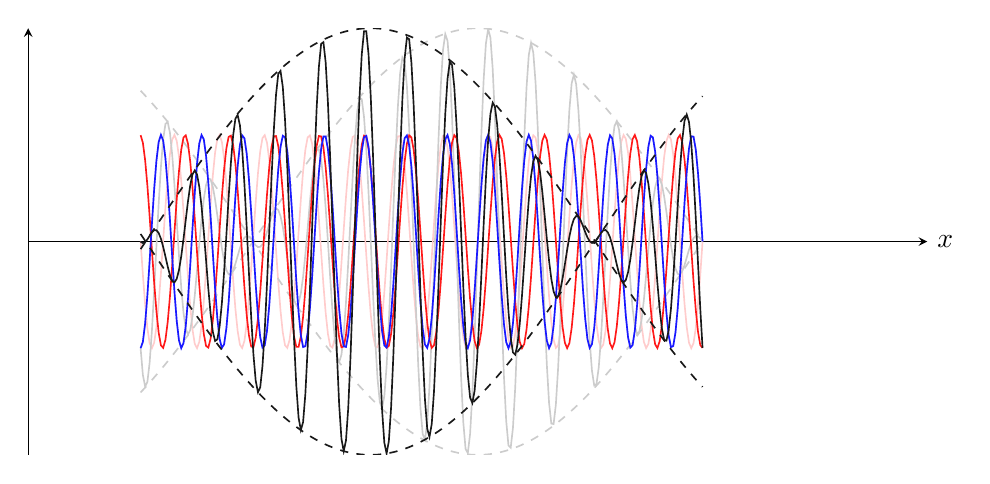
\begin{tikzpicture}
\begin{axis}[
    width=13cm, 
    height=7cm,
    axis x line=center, 
    axis y line=middle, 
    xlabel={$x$},
     x label style={at={(current axis.right of origin)}, right},
    samples=250,
    ymin=-2, ymax=2,
    xmin=0, xmax=20,
    domain=2.5:15,
    ticks=none
]
\addplot [mark=none, semithick, red!20!white] {sin(deg(2*pi*x))};
\addplot [mark=none, semithick, blue!20!white] {sin(deg(2*pi*x*1.1))};
\addplot [mark=none, semithick, black!20!white] {sin(deg(2*pi*x))+sin(deg(2*pi*x*1.1))};
\addplot [mark=none, semithick, dashed, black!20!white] { 2*cos(deg(2*pi*x*0.05))};
\addplot [mark=none, semithick, dashed, black!20!white] {-2*cos(deg(2*pi*x*0.05))};
%
\addplot [mark=none, semithick, red!90!white] {sin(deg(2*pi*x-1.5))};
\addplot [mark=none, semithick, blue!90!white] {sin(deg(2*pi*x*1.1))};
\addplot [mark=none, semithick, black!90!white] {sin(deg(2*pi*x-1.5))+sin(deg(2*pi*x*1.1))};
\addplot [mark=none, semithick, dashed, black!90!white] { 2*cos(deg(2*pi*x*0.05+0.75))};
\addplot [mark=none, semithick, dashed, black!90!white] {-2*cos(deg(2*pi*x*0.05+0.75))};
\end{axis}
\end{tikzpicture}

\caption*{Welle größerer Wellenlänge nach rechts $\leadsto$ Einhüllende nach links}
\end{figure}
}

\end{frame}


\begin{frame}
\frametitle{Dispersion -- Konsequenzen}
  Beliebige Wellenpakete lassen sich durch harmonische Wellen approximieren (siehe Fourier-Transformation), aber wir müssen nun zwischen \textbf{Phasengeschwindigkeit} und \textbf{Gruppengeschwindigkeit} unterscheiden.

\vspace{-7cm}  
\begin{figure}
\hspace{5cm}\animategraphics[draft,loop,autoplay]{10}{ani_img/mikomma/impnorm-}{0}{49}

\vspace{3cm}

\caption*{Rechteckiges Wellenpaket in einem dispersiven Medium \href{http://www.mikomma.de/optik/disp/dispimp.htm}{[mikomma]}}
\end{figure}
\end{frame}


\begin{frame}
\frametitle{Phasengeschwindigkeit}
Harmonische Wellen \hfill
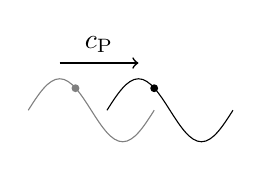
\begin{tikzpicture}[scale=2]
\draw[gray] ( 0.0, 0) sin ( 0.2, 0.2) cos ( 0.4, 0) sin ( 0.6,-0.2) cos ( 0.8, 0);
\fill[gray] (0.3, 0.14) circle[radius=0.025];
\draw ( 0.5, 0) sin ( 0.7, 0.2) cos ( 0.9, 0) sin ( 1.1,-0.2) cos ( 1.3, 0);
\fill (0.8, 0.14) circle[radius=0.025];
\draw[->, semithick] ( 0.2, 0.3) -- node[above] {$c_\mathrm{P}$} (0.7, 0.3);
\end{tikzpicture}

 \begin{equation*}
  w(z,t)=\hat{w} e^{i(\kappa z-\omega t)}
 \end{equation*}
 breiten sich mit der Phasengeschwindigkeit
 \begin{equation*}
  c_\mathrm{P}=\frac{\omega}{\kappa}
 \end{equation*}
 aus, 
wobei eine der beiden Größen, $\omega$ oder $\kappa$, durch die Dispersionbeziehung bestimmt ist.
\end{frame}


\begin{frame}
\frametitle{Gruppengeschwindigkeit}
Für ein Wellenpaket mit Spektrum $W(k)$ \hfill
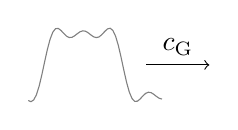
\begin{tikzpicture}[scale=1, domain=-0.2:1.5, samples=50]
\draw[gray] plot (\x,{0.5*sin(\x*180)+(0.5/3)*sin(\x*180*3)+(0.5/5)*sin(\x*180*5))});
\draw[->] (1.3, 0) -- node[above] {$c_\mathrm{G}$} (2.1, 0);
\end{tikzpicture}
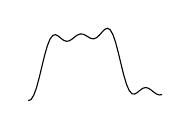
\begin{tikzpicture}[scale=1, domain=-0.2:1.5, samples=50]
\draw plot (\x,{0.45*sin(\x*180)+(0.45/3)*sin(\x*180*3+15)+(0.45/5)*sin(\x*180*5+30))});
\end{tikzpicture}

\begin{equation*}
  w(z,t)=\frac{1}{2\pi}\int_\infty^{+\infty} W(k)e^{i(\kappa z-\omega t)}\mathrm{d}k
 \end{equation*}
 lautet die Gruppengeschwindigkeit
 \begin{equation*}
  c_\mathrm{G}=\frac{\mathrm{d}\omega}{\mathrm{d}\kappa},
 \end{equation*}
wobei $\omega(\kappa)$ durch die Dispersiongleichung bestimmt ist.

\vfill
Knobelspaß: Herleitung 
\end{frame}


\begin{frame}
\frametitle{Dispersionsbeziehung}
\begin{figure}
\begin{tikzpicture}
 \draw[->] (-1,0) -- (10,0) node[right] {$\kappa$};
 \draw[->] (0,-0.5) -- (0,5) node[above] {$\omega$};
 \draw (0,0) .. controls (3,4) and (8,4.5) .. (10,5);
 \draw (5,3.68) circle[radius=0.04];
 \draw[dashed] (0,0) -- node[below,sloped] {$c_\mathrm{P}=\frac{\omega}{\kappa}$} (5,3.68);
 \draw[dashed] (3,2.89) -- node[above,sloped] {$c_\mathrm{G}=\frac{\mathrm{d}\omega}{\mathrm{d}\kappa}$} (7,4.47);
\end{tikzpicture}

\caption*{Phasen- und Gruppengeschwindigkeit}
\end{figure}
\end{frame}


\begin{frame}
\frametitle{Dispersion -- Beispiel 0/3} 
\begin{tikzpicture}
\draw (-1.1, 0) -- (-0.9, 0);
\draw[->] (-1, 0) -- (-1, -1) node[below] {$z$};
\foreach \y in {0,-0.5,...,-4.5}
{
   \draw[<-] (-0.33,\y) -- +(0,-0.45);
   \draw[<-] ( 0.33,\y) -- +(0,-0.45);
}
\draw[->, very thick] (0,1) -- node[right] {$F(t)$} (0,0);
\draw[thick, fill=black!10!white] (-0.25,-5) rectangle (0.25,0);
\draw (0, -5) pic [scale=0.5, thick, rotate=90] {DKbase};
\end{tikzpicture}

\end{frame}


\begin{frame}
\frametitle{Dispersion -- Beispiel 1/3} 
\begin{columns}
  \begin{column}[t]{.6\linewidth}
    \begin{figure}
      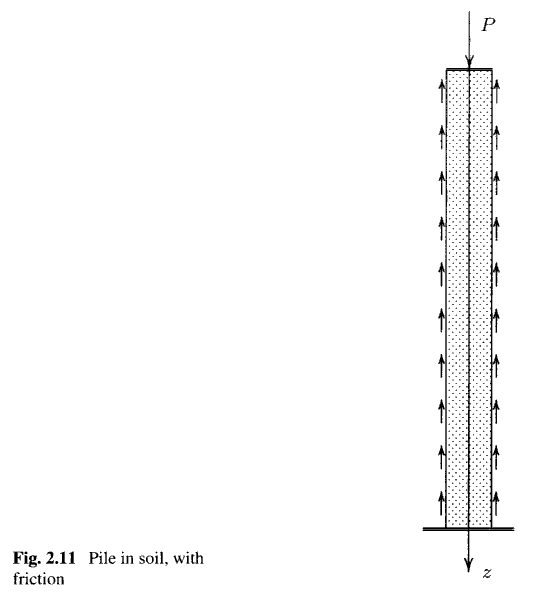
\includegraphics[width=0.65\textwidth]{fig_tikz/wavebar_friction}
      \caption*{Dehnstab mit äußerer, verteilter Steifigkeit~\cite{Verruijt2010}}
    \end{figure}   
  \end{column}
\begin{column}[t]{.4\linewidth}
Bewegungsgleichung
   \begin{align*}
    \rho A \ddot{w}-EAw''+\frac{EA}{H^2}w &= 0 \\
    \ddot{w}-c^2w''+\frac{c^2}{H^2}w &= 0
   \end{align*}
   Harmonischer Wellenansatz
   \begin{align*}
    w&=\hat{w}e^{i(\kappa z-\omega t)}\\
    w''&=-\kappa^2 \hat{w}e^{i(\kappa z-\omega t)}\\
    \ddot{w}&=-\omega^2 \hat{w}e^{i(\kappa z-\omega t)}
   \end{align*}
  \end{column}
\end{columns}
\end{frame}

\begin{frame}
\frametitle{Dispersion -- Beispiel 2/3} 
Einsetzen des Ansatzes in die Bewegungsgleichung
\begin{equation*}
 \left(-\omega^2+\kappa^2 c^2+\frac{c^2}{H^2} \right)\hat{w}e^{i(\kappa z-\omega t)}=0 
\end{equation*}
 liefert die Dispersionbeziehung
\begin{equation*}
 \frac{\omega^2}{\kappa^2}=c^2+\frac{c^2}{\kappa^2 H^2}.
\end{equation*}
Daraus folgen Phasen- und Gruppengeschwindigkeit
\begin{align*}
 c_\mathrm{P}&=c\,\sqrt{1+(\kappa H)^{-2}}, \\
 c_\mathrm{G}&=\frac{c}{\sqrt{1+(\kappa H)^{-2}}}.
\end{align*}
\end{frame}

\begin{frame}
\frametitle{Dispersion -- Beispiel 3/3} 
\begin{figure}
\begin{tikzpicture}
\begin{axis}[
    width=13cm, 
    height=6.5cm,
    axis x line=center, 
    axis y line=middle, 
    xlabel={$\kappa H$},
    x label style={at={(current axis.right of origin)}, right},
    ylabel={},
    y label style={at={(current axis.above origin)}, above},
    samples=100,
    ymin=0, ymax=4.1,
    xmin=0, xmax=5,
    domain=0:5,
]
\addplot [mark=none, semithick] {sqrt(1+1/(x^2))};
\addplot [mark=none, dashed] {1};
\addplot [mark=none, semithick] {1/sqrt(1+1/(x^2))};
\draw (axis cs: 4.75, 1.5) node {$\dfrac{c_\mathrm{P}}{c}$};
\draw (axis cs: 4.75, 0.5) node {$\dfrac{c_\mathrm{G}}{c}$};
\end{axis}
\end{tikzpicture}

\caption*{Phasen- und Gruppengeschwindigkeit in Abhängigkeit der Wellenzahl}
\end{figure}
\end{frame}

\begin{frame}
\frametitle{Dämpfung 1/2}
Die Bewegungsgleichung mit \alert{innerer Dämpfung} lautet
\begin{equation*}
\rho A \ddot{w} - EA w'' \alert{-t_\mathrm{r} EA \dot{w}''}=0,
\end{equation*}
und der Ansatz $w=\hat{w}e^{i(\kappa z-\omega t)}$ liefert die Dispersionbeziehung
\begin{equation*}
 -\omega^2+c^2\kappa^2-i\omega\kappa^2t_\mathrm{r}c^2=0.
\end{equation*}
Die komplexe, frequenzabhängige Wellenzahl
\begin{equation*}
\kappa=\pm \frac{\omega}{c}\sqrt{\frac{1+i\omega t_\mathrm{r}}{1+\omega^2t_\mathrm{r}^2}}=\pm\bigl(\kappa_\mathrm{R}(\omega)+i\kappa_\mathrm{I}(\omega)\bigr)
\end{equation*}
beschreibt Dispersion und Abklingen der Wellen
\begin{equation*}
 w(z,t)=\hat{w}_\mathrm{left}e^{i\bigl(-\kappa_\mathrm{R}(\omega) z-\omega t\bigr)}e^{\kappa_\mathrm{I}(\omega) z}
 +\hat{w}_\mathrm{right}e^{i\bigl(\kappa_\mathrm{R}(\omega) z-\omega t\bigr)}e^{-\kappa_\mathrm{I}(\omega) z} .
\end{equation*}
\end{frame}

\begin{frame}
\frametitle{Dämpfung 2/2}
Die Bewegungsgleichung mit \alert{äußerer Dämpfung} lautet
\begin{equation*}
\rho A \ddot{w} - EA w'' \alert{+ \frac{\rho A}{t_\mathrm{r}}\dot{w}}=0.
\end{equation*}
Mit dem gleichen Ansatz wie zuvor erhalten wir
\begin{align*}
 0 &= -\omega^2+c^2\kappa^2-i\frac{\omega}{t_\mathrm{r}} , \\
\kappa &= \pm \frac{\omega}{c}\sqrt{1+\frac{i}{\omega t_\mathrm{r}}}=\pm\bigl(\kappa_\mathrm{R}(\omega)+i\kappa_\mathrm{I}(\omega)\bigr) , \\
w(z,t)&=\hat{w}_\mathrm{left}e^{i\bigl(-\kappa_\mathrm{R}(\omega) z-\omega t\bigr)}e^{\kappa_\mathrm{I}(\omega) z}
 +\hat{w}_\mathrm{right}e^{i\bigl(\kappa_\mathrm{R}(\omega) z-\omega t\bigr)}e^{-\kappa_\mathrm{I}(\omega) z} .
\end{align*}
\textbf{Anmerkung:} Dämpfung ist meist vernachlässigbar, weil im 3D andere Effekte dominieren (Abklingen durch räumliche Ausbreitung, Dispersion durch tiefenabhängige Elastizität). 
\end{frame}

\subsection{1.5D Erdbebenmodell}

\begin{frame}
\frametitle{Meine Skizze}
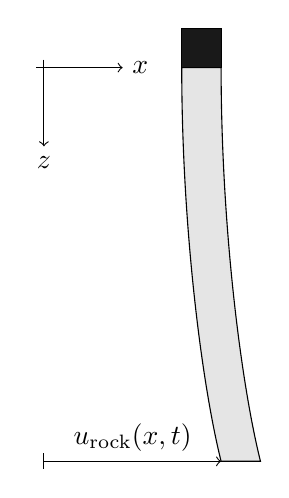
\begin{tikzpicture}
\draw[->] (-2.1, 0.0) -- (-1,0) node[right] {$x$};
\draw[->] (-2.0, 0.1) -- (-2,-1) node[below] {$z$};
\draw[fill=black!90!white] (-0.25,0) rectangle (0.25,0.5);
\draw[fill=black!10!white] (-0.25,0) .. controls (-0.25,-2) and (0.0,-4) .. (0.25,-5) 
-- (0.75,-5)  .. controls (0.5,-4) and (0.25,-2) .. (0.25,0) --cycle;
\draw (-2,-4.9) -- (-2,-5.1);
\draw[->] (-2,-5.0) -- node[above] {$u_\mathrm{rock}(x,t)$} (0.25,-5);
\end{tikzpicture}


\end{frame}

\begin{frame}
\frametitle{Geometrie}

\begin{figure}
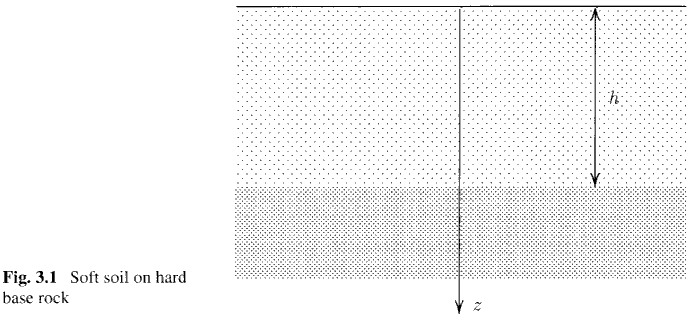
\includegraphics[width=0.67\textwidth]{fig_pdf/earthquake_model}
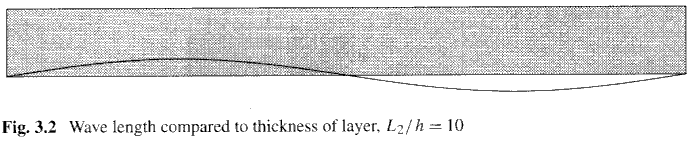
\includegraphics[width=0.7\textwidth]{fig_pdf/earthquake_length_ratio}
\caption*{Bild oben: weiche Bodenschicht auf steifem Felsgrund\\ Bild unten: Erdbebenwellenlänge im Vergleich zu den Abmessungen \cite{Verruijt2010}}
\end{figure}
\end{frame}

\begin{frame}
\frametitle{Bewegungsgleichung}
\begin{figure}
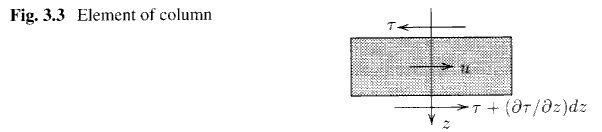
\includegraphics[width=0.7\textwidth]{fig_pdf/earthquake_inf_element}
\caption*{Freischnitt eines infinitesimalen Bodenelements \cite{Verruijt2010}}
\end{figure}
\begin{align*}
 \frac{\partial \tau}{\partial z} &= \rho \frac{\partial^2 u}{\partial t^2}
 \qquad \text{mit} \qquad \tau=\mu \left(\frac{\partial u}{\partial z} +  \frac{\partial w}{\partial x} \right)\approx \mu \frac{\partial u}{\partial z},\\
 \mu \frac{\partial^2 u}{\partial z^2} &= \rho \frac{\partial^2 u}{\partial t^2},\\
 c^2\frac{\partial^2 u}{\partial z^2} &= \frac{\partial^2 u}{\partial t^2}
 \qquad \text{mit} \qquad c^2=\frac{\mu}{\rho}  \qquad \text{\textsl{Wellengleichung :-)}}
\end{align*}
\end{frame}


\begin{frame}
\frametitle{Stationärer Zustand 1/2}
\begin{columns}
\begin{column}[t]{.1\linewidth}
 \begin{tikzpicture}
\draw[->] (0,0) -- ( 1, 0) node[right] {$x$};
\draw[->] (0, 0) -- (0,-6) node[below] {$z$};
\draw[semithick] (0.25, 0) .. controls (0.3, -3) and (0.6,-5) .. (1.1,-6);
 \end{tikzpicture}

\end{column}
\begin{column}[b]{.9\linewidth}
Ansatz
\begin{equation*}
u(x,z,t) = f(z) \sin(\omega t - \kappa_2 x) 
\end{equation*}
Randbedingungen
\begin{align*}
z=0 &:\quad \frac{\partial u}{\partial z}=0\\
z=h &:\quad u=u_0 \sin(\omega t - \kappa_2 x)
\end{align*}
Einsetzen des Ansatzes in die Bewegungsgleichung
\begin{align*}
 c^2 f''+\omega^2 f &=0 \qquad \text{\textsl{Schwingungsgleichung :-)}}\\
 f'(0) &=0\\
 f(h) &= u_0
\end{align*}
\end{column}
\end{columns}
\end{frame}

\begin{frame}
\frametitle{Stationärer Zustand 2/2}
Die allgemeine Lösung der homogenen Differentialgleichung
\begin{equation*}
 f''+\frac{\omega^2}{c^2}f=0,
\end{equation*}
lautet (siehe Einmassenschwinger)
\begin{equation*}
 f(z)=C_1\cos\bigl((\omega/c)z\bigr)+C_2\sin\bigl((\omega/c)z\bigr).
\end{equation*}
Die Konstanten folgen aus den Randbedingungen
\begin{align*}
-C_1(\omega/c)\sin(0)+C_2(\omega/c)\cos(0)&=0 \quad \leadsto \quad C_2=0\\
 C_1\cos\bigl((\omega/c)h\bigr)&=u_0
 \quad \leadsto \quad C_1=\frac{u_0}{\cos\bigl((\omega/c)h\bigr)}
\end{align*}
Als Endergebnis für den gewählten Ansatz erhalten wir
\begin{equation*}
 u(x,z,t)=\frac{u_0}{\cos\bigl((\omega/c)h\bigr)}\cos\bigl((\omega/c)z\bigr)\sin(\omega t - \kappa_2 x) .
\end{equation*}
\end{frame}

\begin{frame}
\frametitle{Berücksichtigung von Auflasten}
\begin{figure}
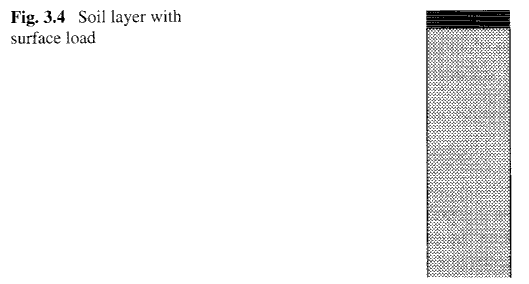
\includegraphics[width=0.525\textwidth]{fig_pdf/earthquake_top_load}
\caption*{Der dunkle Bereich modelliert ein Gebäude \cite{Verruijt2010}}
\end{figure}
\begin{align*}
 z=0 &: \quad \mu\frac{\partial u}{\partial z} = \alert{\rho d \frac{\partial^2 u}{\partial t^2}} \qquad \text{diskrete Randmasse}\\
  u(x,z,t)&=u_0\frac{\cos\bigl((\omega/c)z\bigr)\alert{-d(\omega/c)\sin\bigl((\omega/c)z\bigr)}}{\cos\bigl((\omega/c)h\bigr)\alert{-d(\omega/c)\sin\bigl((\omega/c)h\bigr)}}\sin(\omega t - \kappa_2 x)
\end{align*}
\end{frame}


\begin{frame}
\frametitle{Berücksichtigung innerer Dämpfung 1/2}
Bewegungsgleichung
\begin{equation*}
\frac{\partial^2 u}{\partial t^2} = c^2\frac{\partial^2 u}{\partial z^2} \alert{+ c^2 t_\mathrm{r} \frac{\partial^3 u}{\partial z^2\partial t}}
\end{equation*}
und Randbedingungen
\begin{align*}
 z=0 &: \quad  \mu\frac{\partial u}{\partial z} \alert{+ \mu t_\mathrm{r}  \frac{\partial^2 u}{\partial z\partial t}}= \rho d \frac{\partial^2 u}{\partial t^2} \qquad \text{ohne Auflast} \quad d=0\\
 z=h &: \quad u = u_0 \sin(\omega t - \kappa_2 x)
\end{align*}
Ansatz
\begin{equation*}
 u(x,z,t)=f(z)\sin( \omega t -\kappa_2 x ) \alert{ + g(z)\cos( \omega t -\kappa_2 x)}
\end{equation*}
\end{frame}


\begin{frame}
\frametitle{Berücksichtigung innerer Dämpfung 2/2}

\only<1>{
\begin{figure}
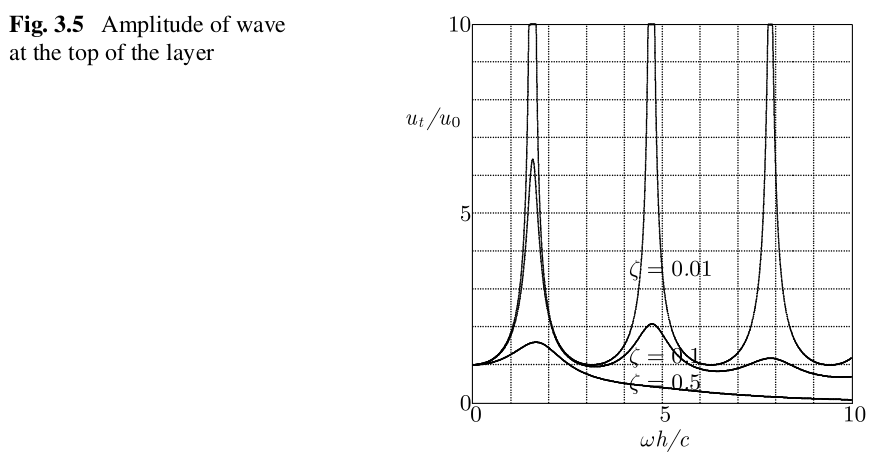
\includegraphics[width=0.8\textwidth]{fig_img/earthquake_damped_amplitude.png}
\caption*{Relative Verschiebungsamplituden an der Oberfläche in Abhängigkeit der dimensionslosen Anregungsfrequenz für verschiedene Dämpfungsgrade  \cite{Verruijt2010}}
\end{figure}
}

\only<2>{
\begin{figure}
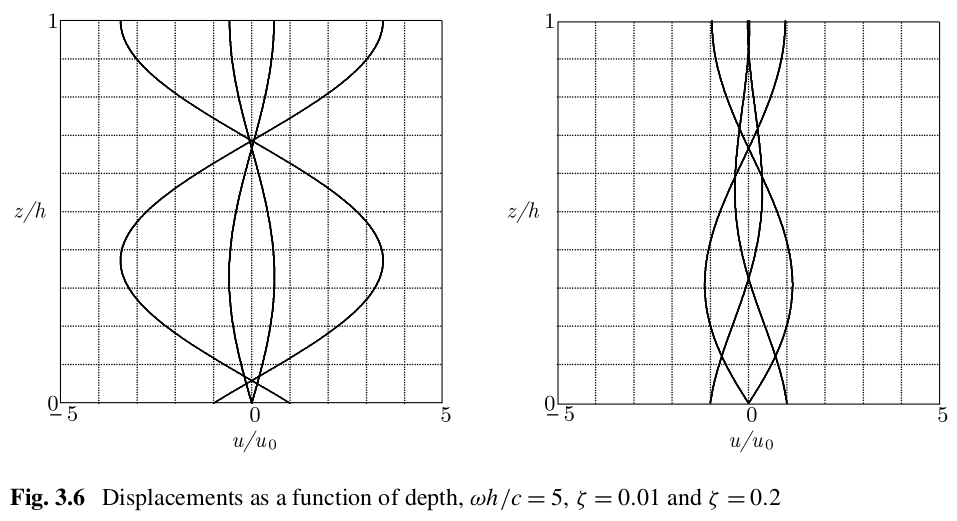
\includegraphics[width=0.85\textwidth]{fig_img/earthquake_damped_displacements.png}
\caption*{Verschiebungsverläufe zu den dimensionslosen Zeiten $\omega t=0$, $\frac{1}{2}\pi$, $\pi$, $\frac{3}{2}\pi$ \cite{Verruijt2010}}
\end{figure}
}
 
\end{frame}

\begin{frame}
\frametitle{Innere Dämpfung und Auflast}

\begin{figure}
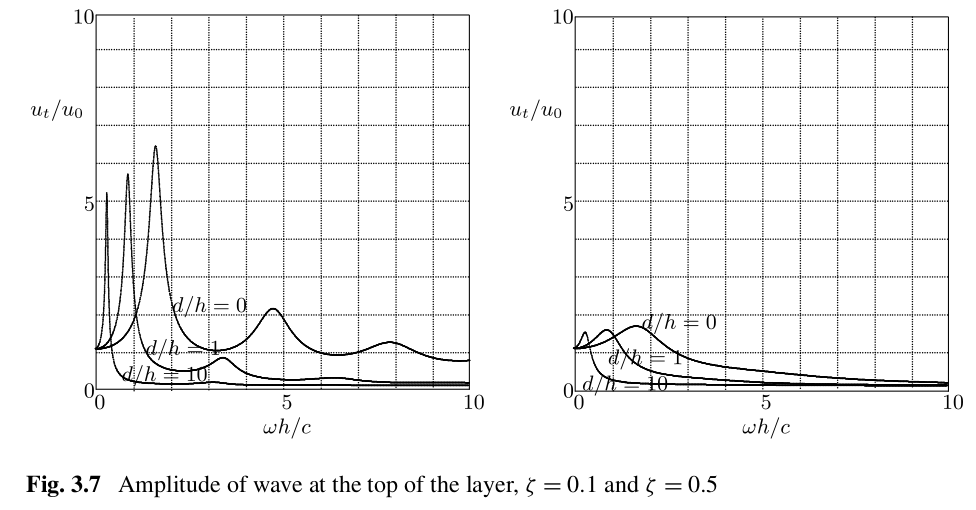
\includegraphics[width=0.85\textwidth]{fig_img/earthquake_damped_top_load.png}
\caption*{Relative Verschiebungsamplituden an der Oberfläche in Abhängigkeit der dimensionslosen Anregungsfrequenz für zwei Dämpfungsgrade und drei Auflasten \cite{Verruijt2010}}
\end{figure}

\end{frame}
